\documentclass[11pt,a4paper]{article}
\usepackage[english]{babel}
\usepackage{graphicx,latexsym,isabelle,isabellesym,amssymb}

% further packages required for unusual symbols (see also
% isabellesym.sty), use only when needed

%\usepackage{amssymb}
  %for \<leadsto>, \<box>, \<diamond>, \<sqsupset>, \<mho>, \<Join>,
  %\<lhd>, \<lesssim>, \<greatersim>, \<lessapprox>, \<greaterapprox>,
  %\<triangleq>, \<yen>, \<lozenge>

%\usepackage{eurosym}
  %for \<euro>

%\usepackage[only,bigsqcap]{stmaryrd}
  %for \<Sqinter>

%\usepackage{eufrak}
  %for \<AA> ... \<ZZ>, \<aa> ... \<zz> (also included in amssymb)

%\usepackage{textcomp}
  %for \<onequarter>, \<onehalf>, \<threequarters>, \<degree>, \<cent>,
  %\<currency>

% this should be the last package used
\usepackage{pdfsetup}

% urls in roman style, theory text in math-similar italics
\urlstyle{rm}
\isabellestyle{it}

% for uniform font size
%\renewcommand{\isastyle}{\isastyleminor}


\begin{document}

\title{Regression Test Selection over JVM}
\author{Susannah Mansky}
\maketitle

\begin{abstract}
This development provides a general definition for safe Regression Test Selection (RTS) algorithms. RTS algorithms select which tests to rerun on revised code, reducing the time required to check for newly introduced errors. An RTS algorithm is considered safe if and only if all deselected tests would have unchanged results.

This definition is instantiated with two class-collection-based RTS algorithms run over the JVM as modeled by JinjaDCI. This is achieved with a general definition for Collection Semantics, small-step semantics instrumented to collect information during execution. As the RTS definition mandates safety, these instantiations include proofs of safety.

This work is described in Mansky and Gunter's LSFA 2020 paper~\cite{MANSKY202051} and Mansky's doctoral thesis~\cite{mansky2020verified}.
\end{abstract}

\tableofcontents

\clearpage
\section{Theory Dependencies}

Figure \ref{theory-deps} shows the dependencies between 
the Isabelle theories in the following sections.

\begin{figure}[h!t]
\begin{center}
  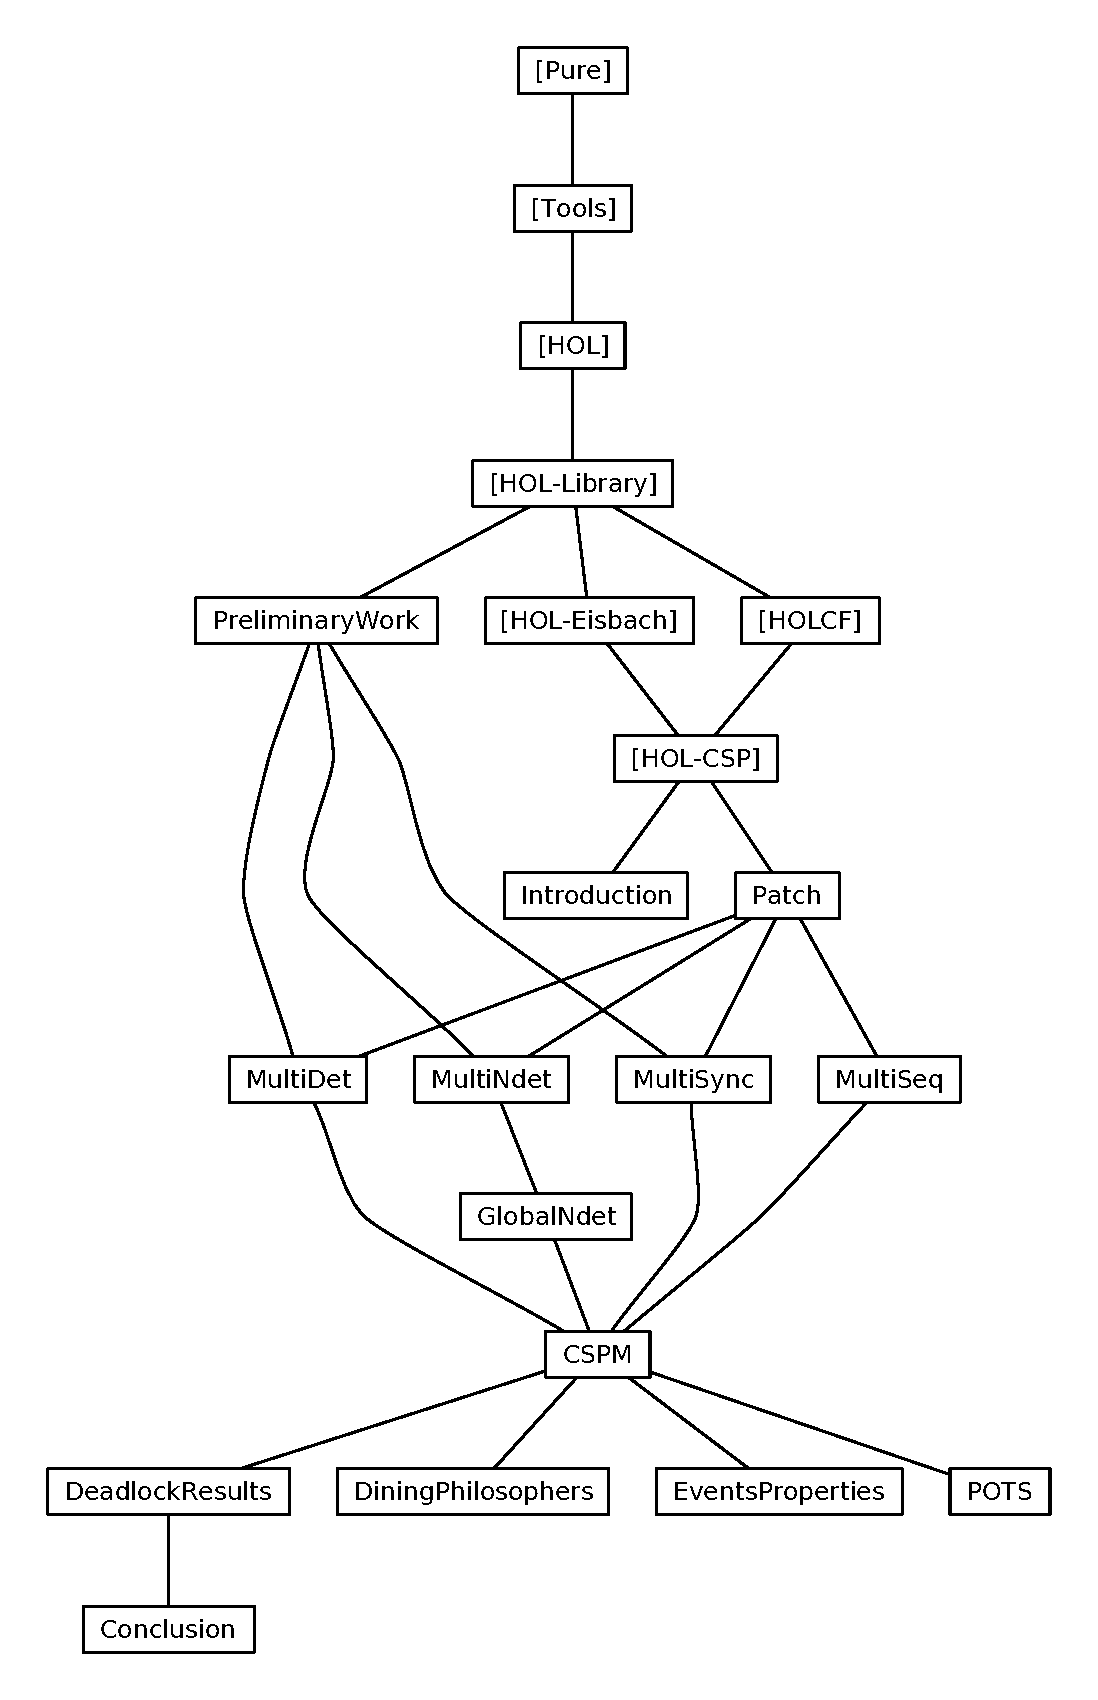
\includegraphics[width=\textwidth]{session_graph}
\end{center}
\caption{Theory Dependency Graph\label{theory-deps}}
\end{figure}

% sane default for proof documents
\parindent 0pt\parskip 0.5ex

% generated text of all theories
\clearpage
\input{session}

% optional bibliography
\bibliographystyle{abbrv}
%\bibliographystyle{plain}
\bibliography{root}

\end{document}

%%% Local Variables:
%%% mode: latex
%%% TeX-master: t
%%% End:
